\documentclass[tikz,border=0pt]{standalone}
\usepackage[T1]{fontenc}
\usepackage{helvet}
\usepackage{amsmath}
\usetikzlibrary{arrows.meta,calc}
\renewcommand{\familydefault}{\sfdefault}

% Standalone vector diagram of SSRB.
\definecolor{ink}{HTML}{18243B}
\definecolor{muted}{HTML}{465570}
\definecolor{border}{HTML}{CDD7E4}
\definecolor{panel}{HTML}{F8FAFD}
\definecolor{mintpanel}{HTML}{F0FCF9}
\definecolor{teal}{HTML}{0F7F78}
\definecolor{cyan}{HTML}{58D7EA}
\definecolor{blue}{HTML}{136FC1}
\definecolor{deepblue}{HTML}{2846A0}
\definecolor{yellow}{HTML}{FFE58A}
\definecolor{orange}{HTML}{F5A21A}
\definecolor{rawfill}{HTML}{FFD4A8}
\definecolor{softblue}{HTML}{AEDCF5}
\definecolor{softmint}{HTML}{90EBDD}
\definecolor{slate}{HTML}{334155}
\definecolor{darkcard}{HTML}{08111F}

\tikzset{
  >={Latex[length=9bp,width=7bp]},
  every node/.style={font=\sffamily\fontsize{11.5}{14}\selectfont,text=muted},
  flow/.style={draw=teal,line width=2.4bp,-{Latex[length=10bp,width=8bp]},
               shorten <=1.5bp,shorten >=1.5bp,line cap=round,line join=round},
  darkflow/.style={draw=slate,line width=1.8bp,-{Latex[length=9bp,width=7bp]},
                   shorten <=1.5bp,shorten >=1.5bp,line cap=round,line join=round},
  thinflow/.style={draw=teal,line width=1.7bp,-{Latex[length=8bp,width=6bp]},
                   shorten <=1.2bp,shorten >=1.2bp,line cap=round,line join=round},
  title/.style={font=\sffamily\bfseries\fontsize{16}{19}\selectfont,
                text=ink,anchor=west},
  heading/.style={font=\sffamily\bfseries\fontsize{13.5}{16}\selectfont,
                  text=ink,align=center},
  label/.style={font=\sffamily\bfseries\fontsize{12.5}{15}\selectfont,
                text=slate,align=center},
  body/.style={font=\sffamily\fontsize{11.5}{14}\selectfont,
               text=muted,align=center},
  tiny/.style={font=\sffamily\fontsize{9.3}{11.2}\selectfont,
               text=muted,align=center},
  box/.style={draw=teal,line width=1.4bp,rounded corners=2bp,align=center},
  smallbox/.style={draw=border,line width=1.1bp,fill=white,
                   rounded corners=3bp,align=center}
}

\begin{document}
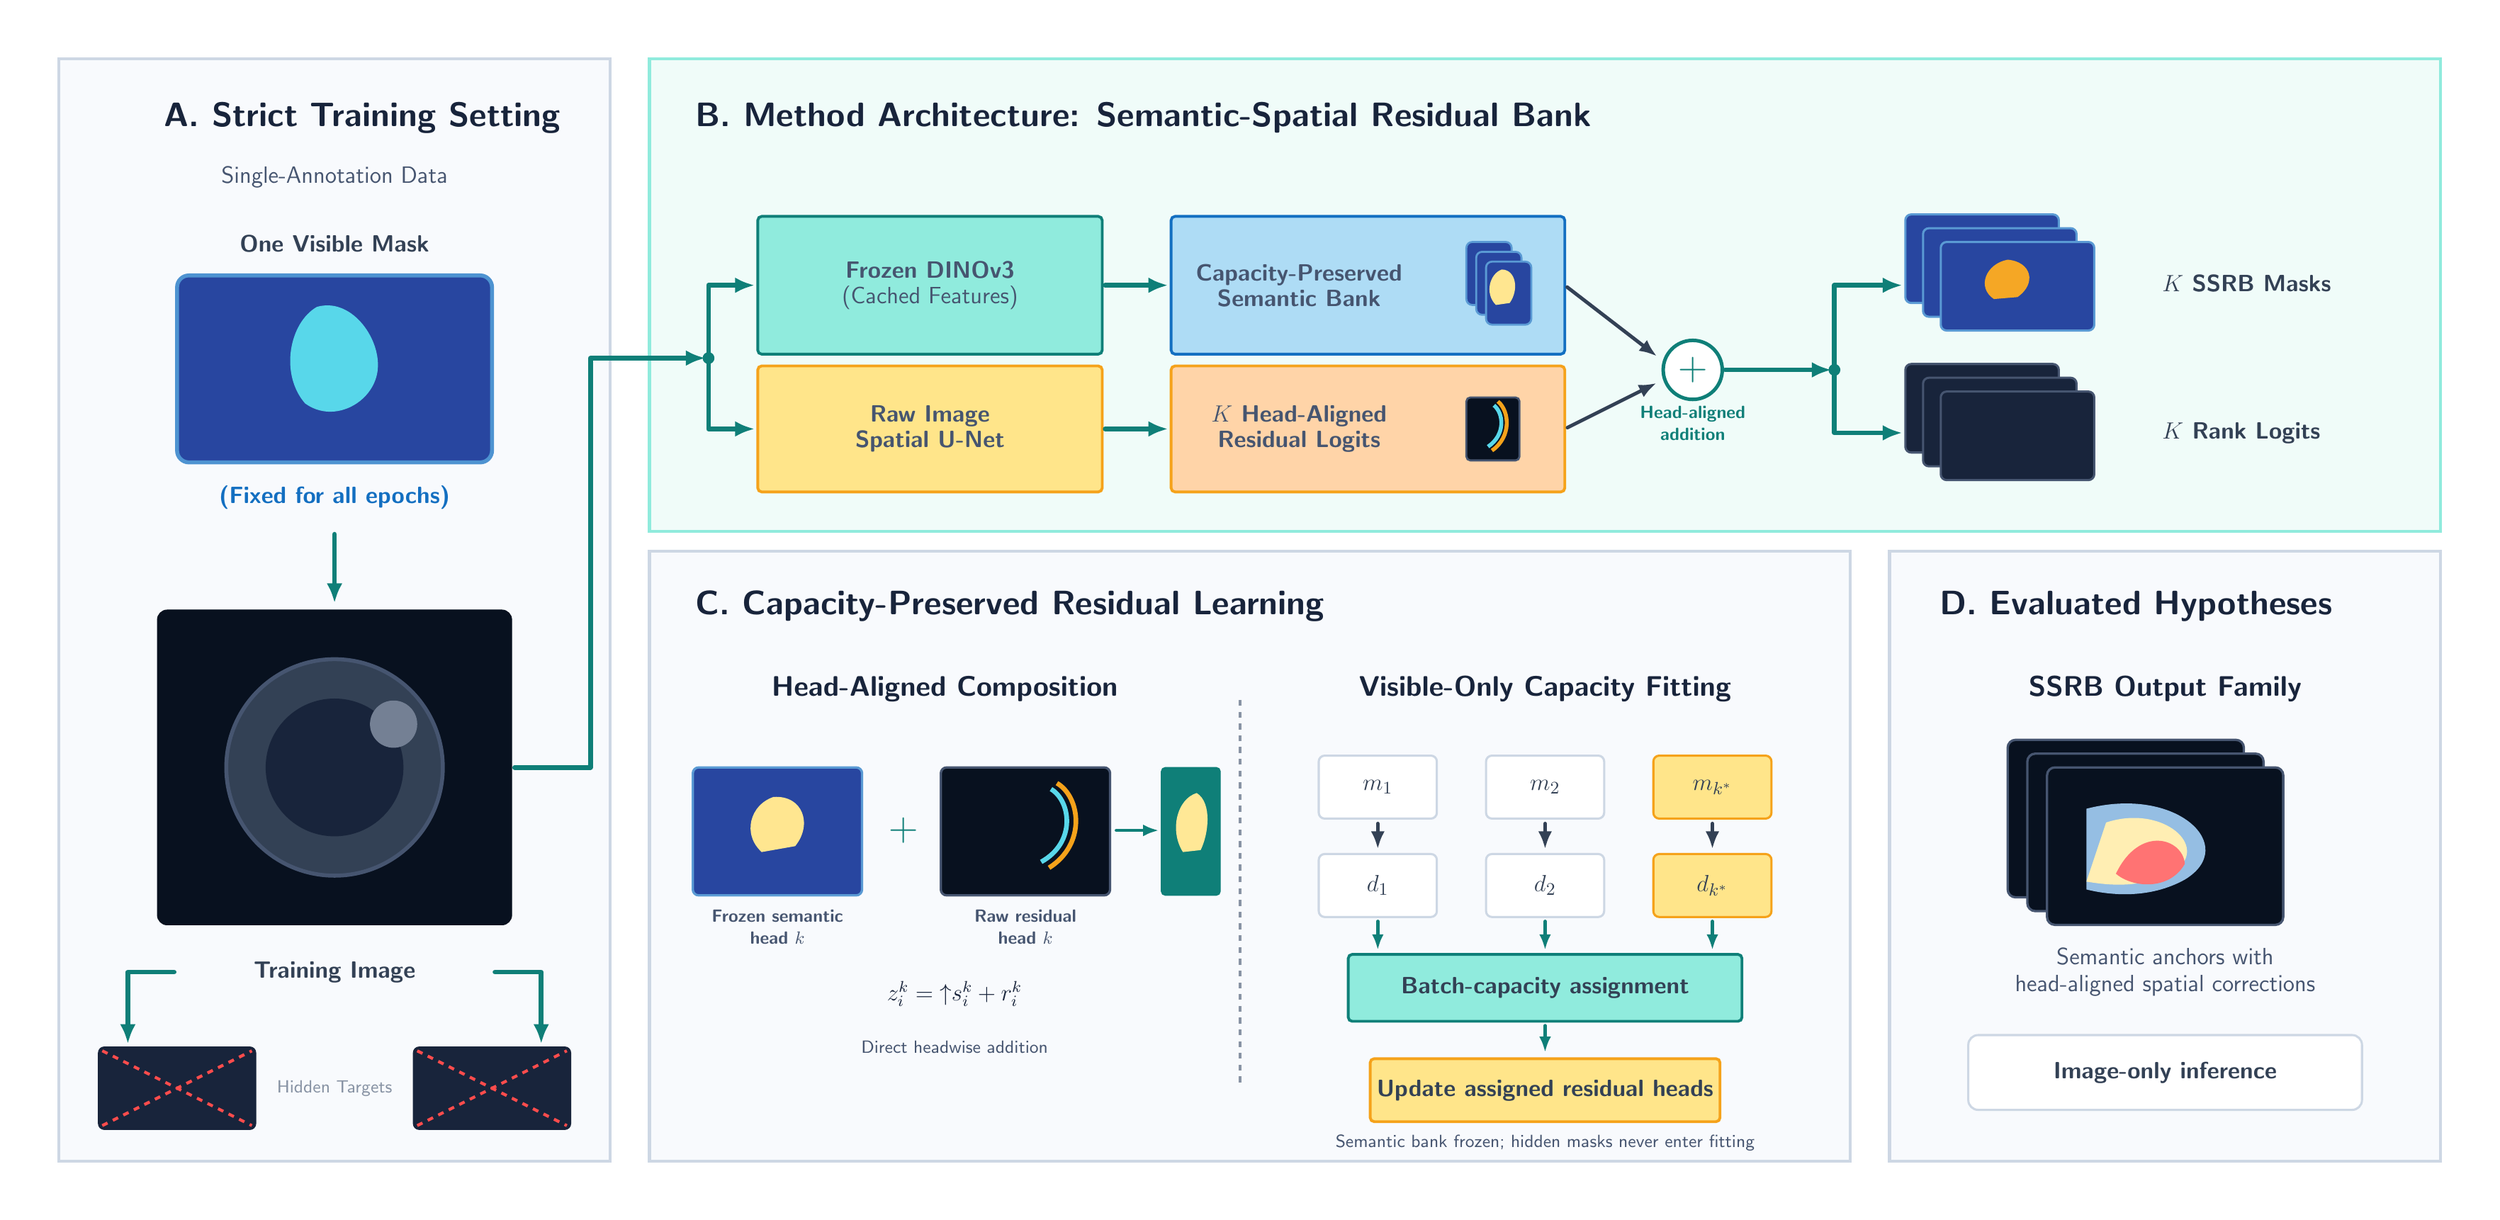
\begin{tikzpicture}[x=1bp,y=1bp]
  \path[use as bounding box] (0,0) rectangle (1250,600);
  \fill[white] (0,0) rectangle (1250,600);

  % Four-panel geometry retained from the reviewed figure.
  \draw[fill=panel,draw=border,line width=1.5bp]
    (20,20) rectangle (300,580);
  \draw[fill=mintpanel,draw=softmint,line width=1.5bp]
    (320,340) rectangle (1230,580);
  \draw[fill=panel,draw=border,line width=1.5bp]
    (320,20) rectangle (930,330);
  \draw[fill=panel,draw=border,line width=1.5bp]
    (950,20) rectangle (1230,330);

  % ---------------------------------------------------------------------
  % A. Strict single-annotation training setting.
  \node[title] at (70,550) {A. Strict Training Setting};
  \node[body] at (160,520) {Single-Annotation Data};
  \node[label] at (160,486) {One Visible Mask};

  \draw[fill=deepblue,draw=blue!75,line width=2bp,rounded corners=6bp]
    (80,375) rectangle (240,470);
  \path[fill=cyan]
    (145,405) .. controls (132,420) and (137,446) .. (151,454)
    .. controls (168,459) and (183,439) .. (182,423)
    .. controls (181,406) and (160,394) .. cycle;
  \node[body,text=blue] at (160,357) {\textbf{(Fixed for all epochs)}};

  \draw[flow] (160,340) -- (160,302);
  \draw[fill=darkcard,draw=darkcard,rounded corners=5bp]
    (70,140) rectangle (250,300);
  \path[fill=slate,draw=muted,line width=2bp] (160,220) circle (55bp);
  \path[fill=ink] (160,220) circle (35bp);
  \path[fill=muted!75] (190,242) circle (12bp);
  \node[label,fill=panel,inner sep=3bp] at (160,116) {Training Image};

  \draw[flow] (80,116) -| (55,78);
  \draw[flow] (240,116) -| (265,78);
  \foreach \xa/\xb in {40/120,200/280}{
    \draw[fill=ink,draw=ink,rounded corners=3bp] (\xa,36) rectangle (\xb,78);
    \draw[red!70,line width=1.5bp,dashed] (\xa+2,38) -- (\xb-2,76);
    \draw[red!70,line width=1.5bp,dashed] (\xa+2,76) -- (\xb-2,38);
  }
  \node[tiny,text=border!55!slate,fill=panel,inner sep=2bp] at (160,57)
    {Hidden Targets};

  % The image enters once and splits cleanly into the two aligned branches.
  \draw[flow] (250,220) -- (290,220) -- (290,428) -- (350,428);
  \fill[teal] (350,428) circle (3bp);
  \draw[flow] (350,428) |- (375,465);
  \draw[flow] (350,428) |- (375,392);

  % ---------------------------------------------------------------------
  % B. Two-branch semantic-spatial residual bank.
  \node[title] at (340,550)
    {B. Method Architecture: Semantic-Spatial Residual Bank};

  \node[box,fill=softmint,minimum width=175bp,minimum height=70bp]
    at (462.5,465)
    {\textbf{Frozen DINOv3}\\[-1bp](Cached Features)};
  \node[box,draw=blue,fill=softblue,minimum width=200bp,minimum height=70bp]
    at (685,465) {};
  \node[body] at (650,465)
    {\textbf{Capacity-Preserved}\\[-1bp]\textbf{Semantic Bank}};

  \draw[flow] (550,465) -- (585,465);

  % Small semantic-head stack inside the semantic-bank block.
  \foreach \dx/\dy in {0/10,5/5,10/0}{
    \draw[fill=deepblue,draw=blue!70,line width=1bp,rounded corners=3bp]
      (735+\dx,445+\dy) rectangle (758+\dx,477+\dy);
  }
  \path[fill=yellow!95]
    (750,455) .. controls (744,461) and (747,471) .. (753,473)
    .. controls (760,473) and (762,463) .. (757,456) -- cycle;

  \node[box,draw=orange,fill=yellow,minimum width=175bp,minimum height=64bp]
    at (462.5,392)
    {\textbf{Raw Image}\\[-1bp]\textbf{Spatial U-Net}};
  \node[box,draw=orange,fill=rawfill,minimum width=200bp,minimum height=64bp]
    at (685,392) {};
  \node[body] at (650,392)
    {\textbf{$K$ Head-Aligned}\\[-1bp]\textbf{Residual Logits}};
  \draw[flow] (550,392) -- (585,392);

  % Residual-logit icon.
  \draw[fill=darkcard,draw=muted,line width=1bp,rounded corners=2bp]
    (735,376) rectangle (762,408);
  \draw[cyan,line width=2bp] (746,383) .. controls (755,389) and (754,400) .. (749,404);
  \draw[orange,line width=2bp] (748,381) .. controls (758,388) and (757,401) .. (751,406);

  % Head-aligned addition.
  \draw[darkflow] (785,465) -- (833,428);
  \draw[darkflow] (785,392) -- (833,416);
  \draw[fill=white,draw=teal,line width=1.8bp] (850,422) circle (15bp);
  \node[font=\sffamily\bfseries\fontsize{22}{24}\selectfont,text=teal]
    at (850,422) {$+$};
  \node[tiny,text=teal] at (850,395) {\textbf{Head-aligned}\\\textbf{addition}};

  % Returned masks and score logits.
  \draw[flow] (865,422) -- (922,422);
  \fill[teal] (922,422) circle (3bp);
  \draw[flow] (922,422) |- (958,465);
  \draw[flow] (922,422) |- (958,390);

  \foreach \dx/\dy in {0/14,9/7,18/0}{
    \draw[fill=deepblue,draw=blue!70,line width=1.1bp,rounded corners=3bp]
      (958+\dx,442+\dy) rectangle (1036+\dx,487+\dy);
  }
  \path[fill=orange!95]
    (1003,458) .. controls (994,464) and (999,476) .. (1010,478)
    .. controls (1022,477) and (1025,466) .. (1015,459) -- cycle;
  \node[label,anchor=west] at (1085,466) {$K$ SSRB Masks};

  \foreach \dx/\dy in {0/14,9/7,18/0}{
    \draw[fill=ink,draw=muted,line width=1.1bp,rounded corners=3bp]
      (958+\dx,366+\dy) rectangle (1036+\dx,411+\dy);
  }
  \node[label,anchor=west] at (1085,390) {$K$ Rank Logits};

  % ---------------------------------------------------------------------
  % C. The aligned residual update under capacity-preserved supervision.
  \node[title] at (340,302) {C. Capacity-Preserved Residual Learning};
  \node[heading] at (470,260) {Head-Aligned Composition};

  \draw[fill=deepblue,draw=blue!70,line width=1.2bp,rounded corners=3bp]
    (342,155) rectangle (428,220);
  \path[fill=yellow!95]
    (377,177) .. controls (367,186) and (371,201) .. (383,205)
    .. controls (398,206) and (403,191) .. (394,180) -- cycle;

  \node[font=\sffamily\bfseries\fontsize{21}{23}\selectfont,text=teal]
    at (449,188) {$+$};
  \draw[fill=darkcard,draw=muted,line width=1.2bp,rounded corners=3bp]
    (468,155) rectangle (554,220);
  \draw[cyan,line width=2.4bp] (519,172) .. controls (537,182) and (534,203) .. (524,209);
  \draw[orange,line width=2.4bp] (523,169) .. controls (542,181) and (539,205) .. (527,212);

  \draw[thinflow] (556,188) -- (580,188);
  \draw[fill=teal,draw=teal,rounded corners=2bp] (580,155) rectangle (610,220);
  \path[fill=yellow!90]
    (591,177) .. controls (584,188) and (588,204) .. (598,207)
    .. controls (606,202) and (604,186) .. (600,178) -- cycle;

  \node[tiny] at (385,139) {\textbf{Frozen semantic}\\\textbf{head $k$}};
  \node[tiny] at (511,139) {\textbf{Raw residual}\\\textbf{head $k$}};
  \node[body,text=ink] at (475,105)
    {$z_i^k=\mathord{\uparrow}s_i^k+r_i^k$};
  \node[tiny] at (475,78) {Direct headwise addition};

  \draw[border!55!slate,line width=1.2bp,dashed]
    (620,60) -- (620,255);

  \node[heading] at (775,260) {Visible-Only Capacity Fitting};

  % Per-head losses and the batch-capacity assignment.
  \foreach \x/\mt/\dt/\fc/\dc in {
    690/{m_1}/{d_1}/white/border,
    775/{m_2}/{d_2}/white/border,
    860/{m_{k^*}}/{d_{k^*}}/yellow/orange}{
    \node[smallbox,fill=\fc,draw=\dc,minimum width=60bp,minimum height=32bp,
          label] (m\x) at (\x,210) {$\mt$};
    \draw[darkflow] (\x,193) -- (\x,177);
    \node[smallbox,fill=\fc,draw=\dc,minimum width=60bp,minimum height=32bp,
          label] (d\x) at (\x,160) {$\dt$};
    \draw[thinflow] (\x,143) -- (\x,126);
  }

  \node[box,fill=softmint,minimum width=200bp,minimum height=34bp,label]
    at (775,108) {Batch-capacity assignment};
  \draw[thinflow] (775,90) -- (775,74);
  \node[box,draw=orange,fill=yellow,minimum width=150bp,
        minimum height=32bp,label] at (775,56)
    {Update assigned residual heads};
  \node[tiny] at (775,29)
    {Semantic bank frozen; hidden masks never enter fitting};

  % ---------------------------------------------------------------------
  % D. Fixed image-only hypothesis family.
  \node[title] at (972,302) {D. Evaluated Hypotheses};
  \node[heading] at (1090,260) {SSRB Output Family};

  \foreach \dx/\dy in {0/14,10/7,20/0}{
    \draw[fill=darkcard,draw=muted,line width=1.2bp,rounded corners=4bp]
      (1010+\dx,140+\dy) rectangle (1130+\dx,220+\dy);
  }
  \path[fill=blue!45]
    (1050,158) -- (1050,199) .. controls (1096,211) and (1128,180) ..
    (1100,163) .. controls (1082,153) and (1062,155) .. cycle;
  \path[fill=yellow!65]
    (1050,162) -- (1060,192) .. controls (1087,201) and (1111,182) ..
    (1097,169) .. controls (1080,158) and (1062,160) .. cycle;
  \path[fill=red!55]
    (1065,166) .. controls (1077,191) and (1099,184) .. (1100,171)
    .. controls (1092,157) and (1073,159) .. cycle;

  \node[body] at (1090,116)
    {Semantic anchors with\\head-aligned spatial corrections};

  \draw[fill=white,draw=border,line width=1.1bp,rounded corners=5bp]
    (990,46) rectangle (1190,84);
  \node[label] at (1090,65) {Image-only inference};

\end{tikzpicture}
\end{document}
